\documentclass[aspectratio=169]{beamer}
\usepackage{natbib}
\usepackage{graphicx}
\graphicspath{{../.}}
\usepackage{tikz}
\usetikzlibrary{positioning}
\usetikzlibrary{calc}
\usepackage{multimedia}
\usepackage{animate}
\usepackage{hyperref}
\usepackage{mathpazo}

\definecolor{cardinalred}{RGB}{140,21,21}
%--- Custom footline
\setbeamertemplate{footline}{%
\begin{beamercolorbox}[wd=\paperwidth,ht=4ex,dp=2.5ex]{}
    \centering
    \makebox[0.32\paperwidth][l]{\scriptsize\texttt{pressure proc. 05-28}}
    \makebox[0.32\paperwidth][c]{\scriptsize\texttt{$^{\dag}$masseyj@stanford.edu}}
    \makebox[0.32\paperwidth][r]{\scriptsize\insertframenumber/\inserttotalframenumber}
  \end{beamercolorbox}
}

\definecolor{cardinalred}{RGB}{140,21,21}
\definecolor{coolgray}{RGB}{77,79,83}
\definecolor{black}{RGB}{0,0,0}
\definecolor{beige}{RGB}{210,194,149}
\definecolor{darkbeige}{RGB}{179,153,93}
\definecolor{darkcardinal}{RGB}{94,48,50}
\definecolor{lightcardinal}{RGB}{141,60,30}
\definecolor{darkpurple}{RGB}{83,40,79}
\definecolor{darkcyan}{RGB}{0,124,146}
\definecolor{skyblue}{RGB}{0,152,219}
\definecolor{treegreen}{RGB}{0,155,118}
\definecolor{darkorange}{RGB}{168,101,12}
\definecolor{beigegray}{RGB}{95,87,79}
\definecolor{boxgray}{RGB}{238,235,233}
\definecolor{footergray}{RGB}{199,209,197}



\mode<presentation>

\setbeamercolor*{palette primary}{use=structure,fg=white,bg= cardinalred}
\setbeamercolor*{palette secondary}{use=structure,fg=white,bg= coolgray}
\setbeamercolor*{palette tertiary}{use=structure,fg=white,bg= darkcardinal}
\setbeamercolor*{palette quaternary}{fg=white,bg= darkbeige}

\setbeamercolor*{sidebar}{use=structure,bg= beige}
\setbeamercolor*{footer}{use=structure,bg= footergray,fg=darkcardinal}
  
\setbeamercolor*{palette sidebar primary}{use=structure,fg=structure.fg!10}
\setbeamercolor*{palette sidebar secondary}{fg=white}
\setbeamercolor*{palette sidebar tertiary}{use=structure,fg=structure.fg!50}
\setbeamercolor*{palette sidebar quaternary}{fg=white}

\setbeamercolor*{titlelike}{parent=palette primary}
\setbeamercolor*{foot line}{parent=palette secondary}

\setbeamercolor*{separation line}{}
\setbeamercolor*{fine separation line}{}

\setbeamercolor{itemize item}{fg=cardinalred}
\setbeamercolor{itemize subitem}{fg=cardinalred}
\setbeamercolor{itemize subsubitem}{fg=cardinalred}
\setbeamercolor{enumerate item}{fg=cardinalred}
\setbeamercolor{enumerate subitem}{fg=cardinalred}
\setbeamercolor{enumerate subsubitem}{fg=cardinalred}
\setbeamercolor{description item}{fg=cardinalred}

\setbeamertemplate{bibliography item}[text]
\setbeamertemplate{frametitle continuation}[from second]
\setbeamercolor{bibliography entry title}{fg=black}
\setbeamercolor{bibliography entry author}{fg=black}
\setbeamercolor*{bibliography entry location}{fg=black}
\setbeamercolor*{bibliography entry note}{fg=black}

\renewcommand*{\bibfont}{\small}
\setbeamertemplate{navigation symbols}{}

\setbeamerfont{footnote}{size=\tiny}

\mode
<all>

\newcommand{\Rt}{\mathit{Re}_{\tau}}
\newcommand{\Rey}{\mathit{Re}}

%--- Title info
\title{Pressure signal processing}
\author{JMO Massey$^{\dag}$, F Cabrera-Booman, T Jaroslawski, J Klewicki, BJ McKeon}
\institute{Center for Turbulence Research \\ Stanford University}
% \thanks{This work was supported by DARPA under the CHAOS program}
\date{April 4, 2025}

\begin{document}

%--- Title page
\begin{frame}
    \setcounter{framenumber}{0}
    \titlepage
    \vfill
    {\scriptsize \centering Thanks to DARPA for funding this work.\par}
\end{frame}

\begin{frame}{Match mics by finding the complex transfer function}
    \centering
    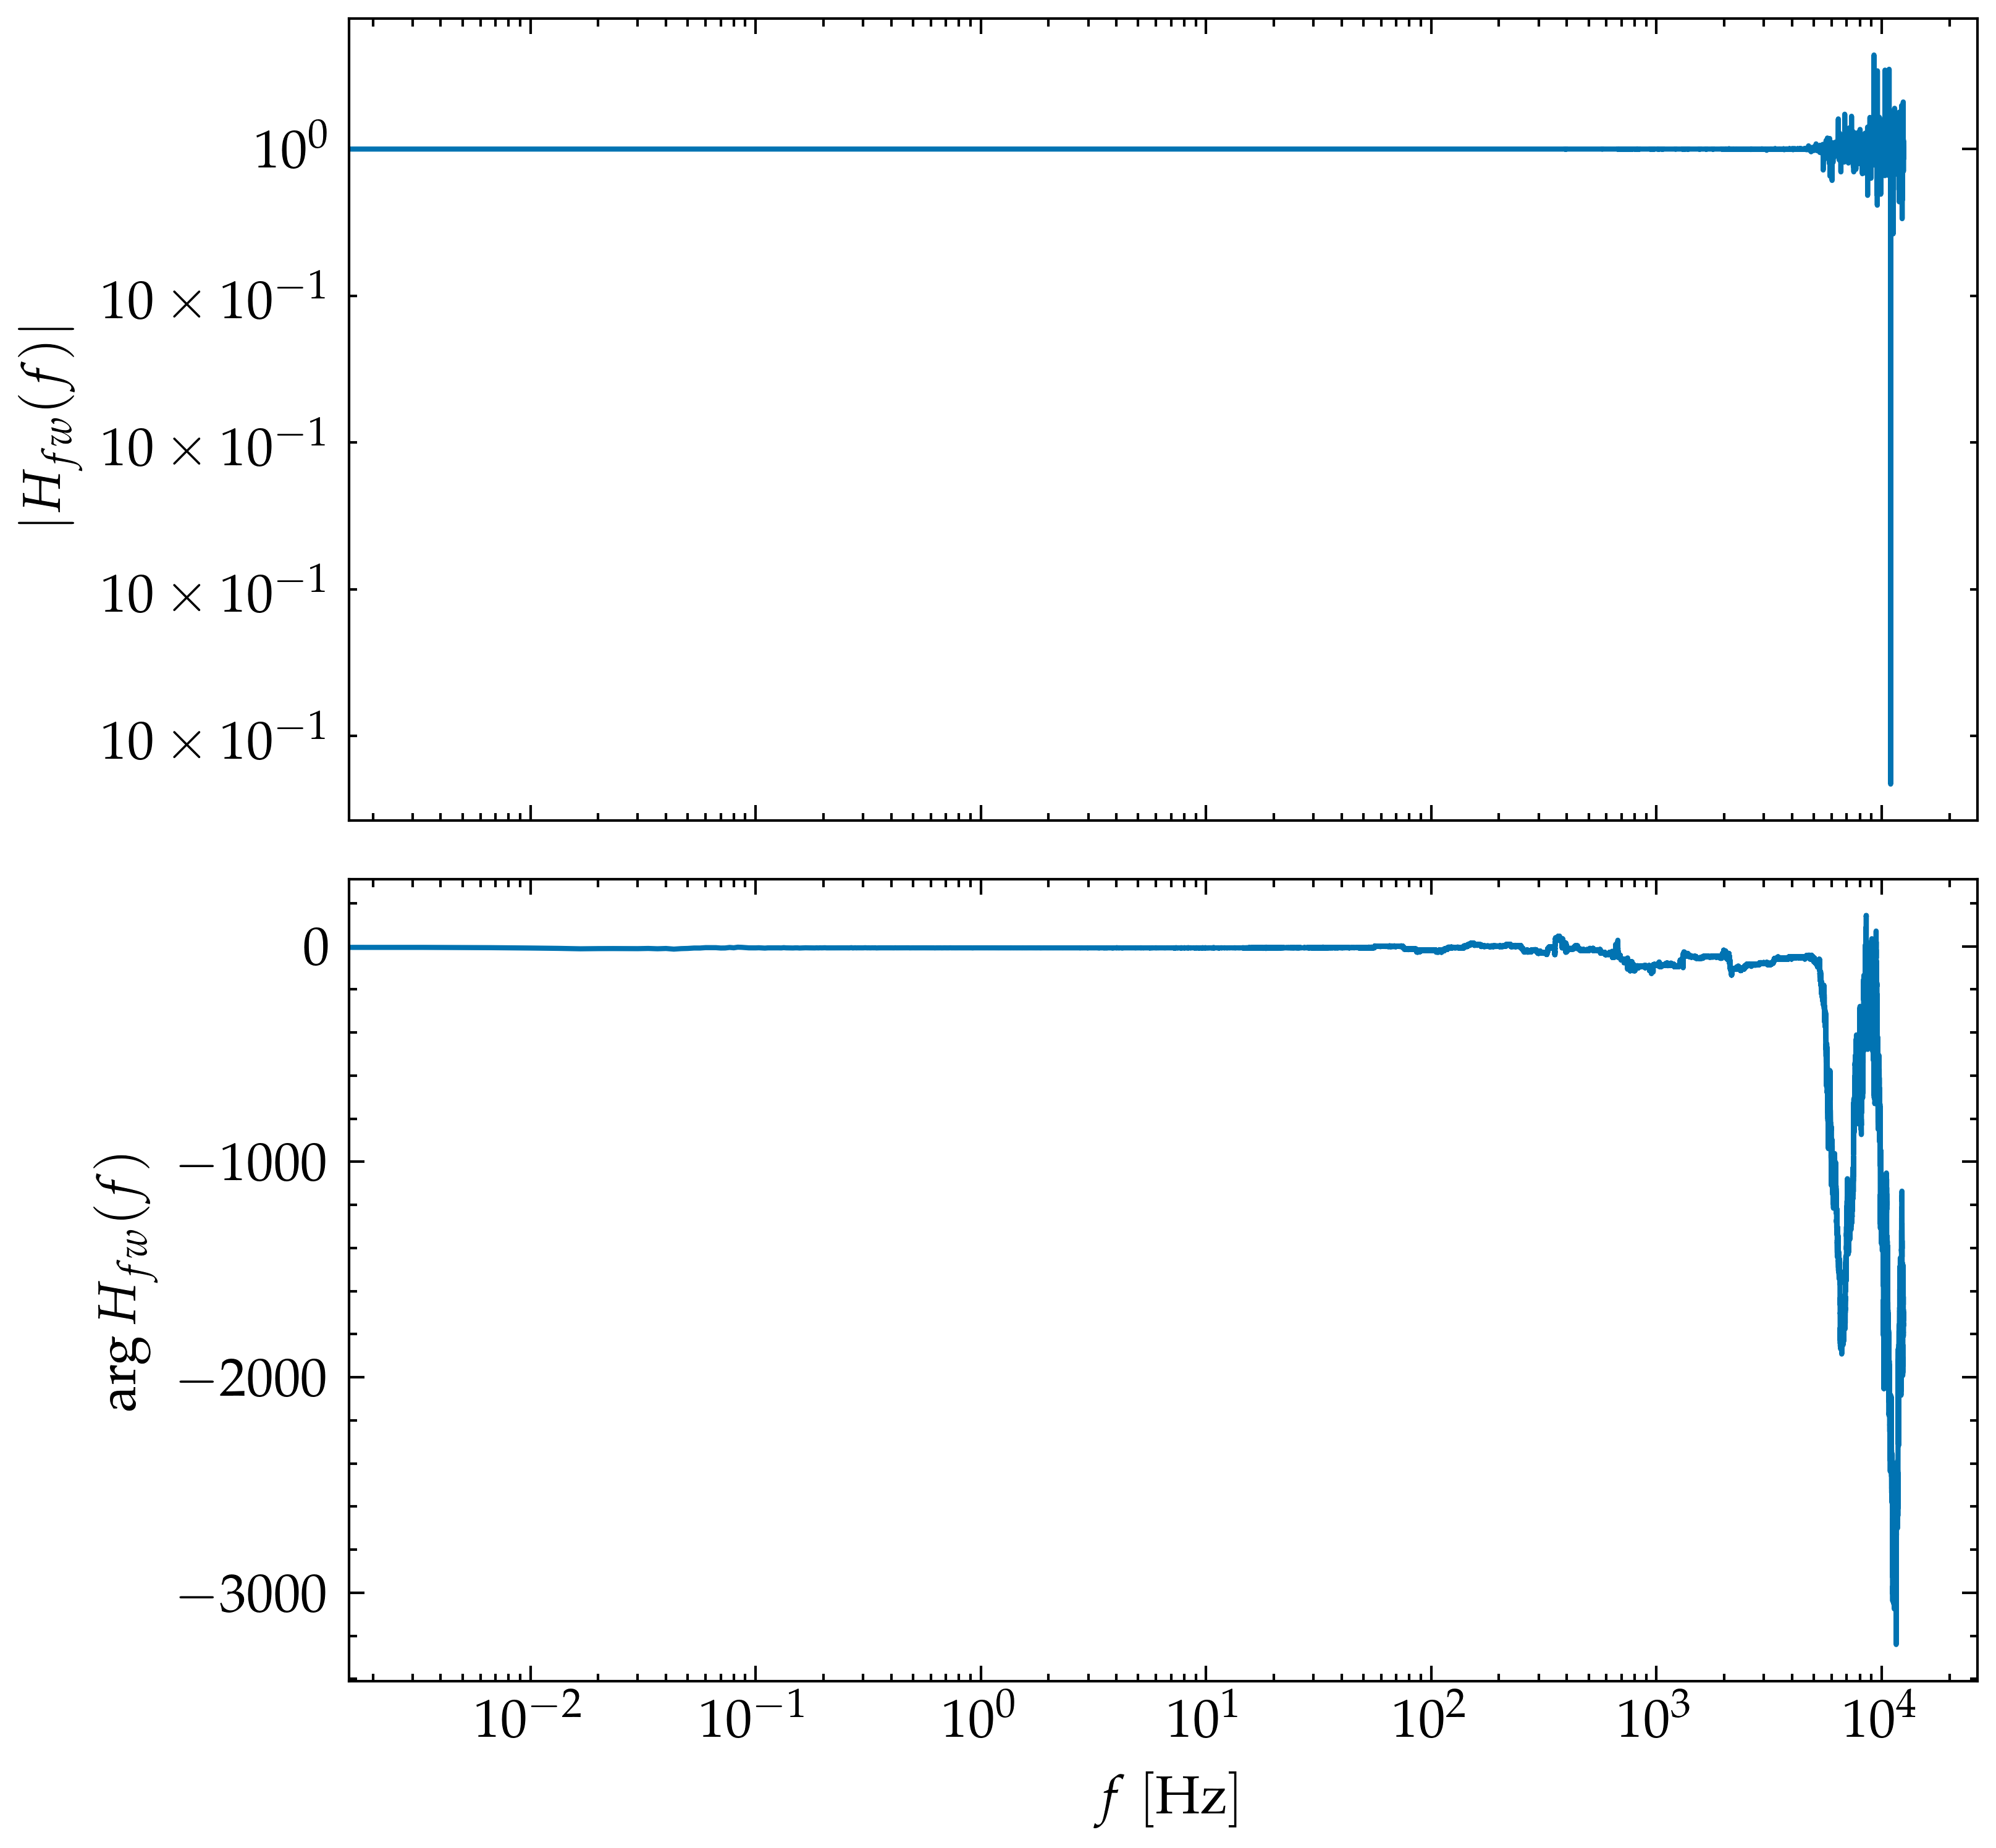
\includegraphics[width=0.7\linewidth]{figures/complex_transfer_function.png}
    \begin{itemize}
            \centering
        \item The microphones aren't phase matched
        \item Here, we match the phase response of the fs and wall measurements to approximate the complex transfer function
        \item $argH_{fw}(f)$ \emph{should} be found in an anechoic chamber with a known input signal
    \end{itemize}
\end{frame}

\begin{frame}{Phase matching dramatically increases the coherence}
    \centering
    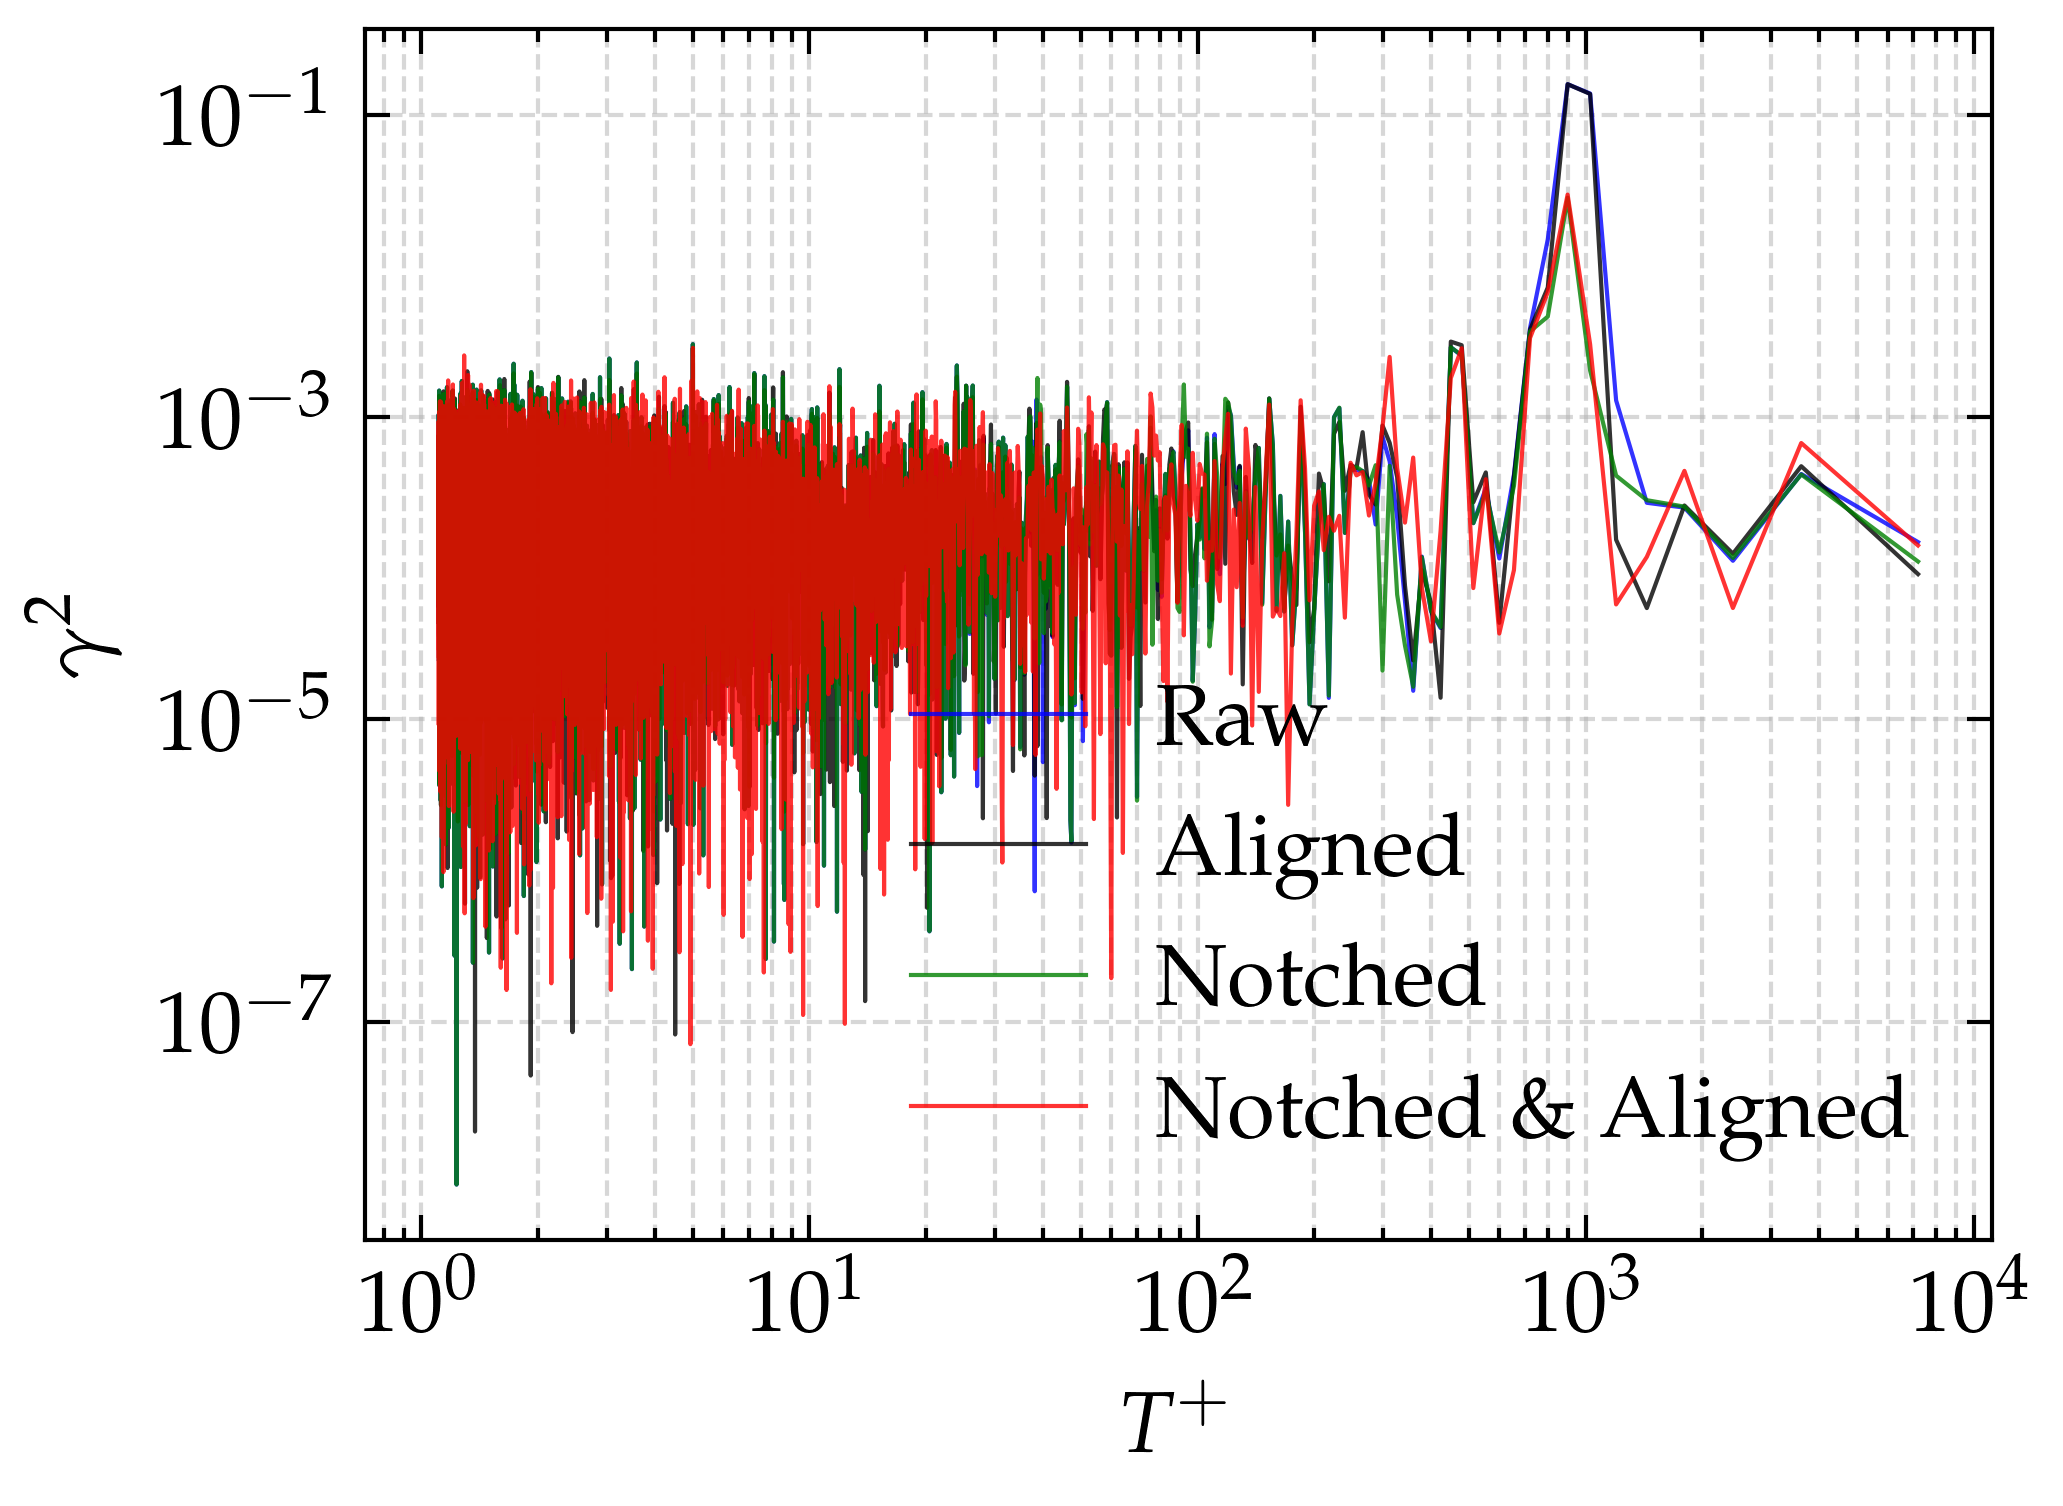
\includegraphics[width=0.7\linewidth]{figures/coherence.png}
    \begin{itemize}
        \centering
        \item Without the complex transfer function, the coherence is very low
        \item The magnitude of the transfer function between fs and wall measurements needs to be determined
        \item We \emph{assume} it is unity for the purposes of this analysis
    \end{itemize}
\end{frame}

\begin{frame}{Wiener filter}
    The Wiener filter is used to reject free-stream noise from the wall-pressure measurements. It has equation
    \begin{equation}
        H_{\text{Wiener}}(f) = \frac{P_{fw}(f)}{P_{ww}(f)}
    \end{equation}
    where $P_{fw}(f)$ is the cross spectral density between the reference and wall pressure signals, and $P_{ww}(f)$ is the power spectral density of the wall pressure signal.
    \begin{minipage}{0.6\textwidth}
        \centering
        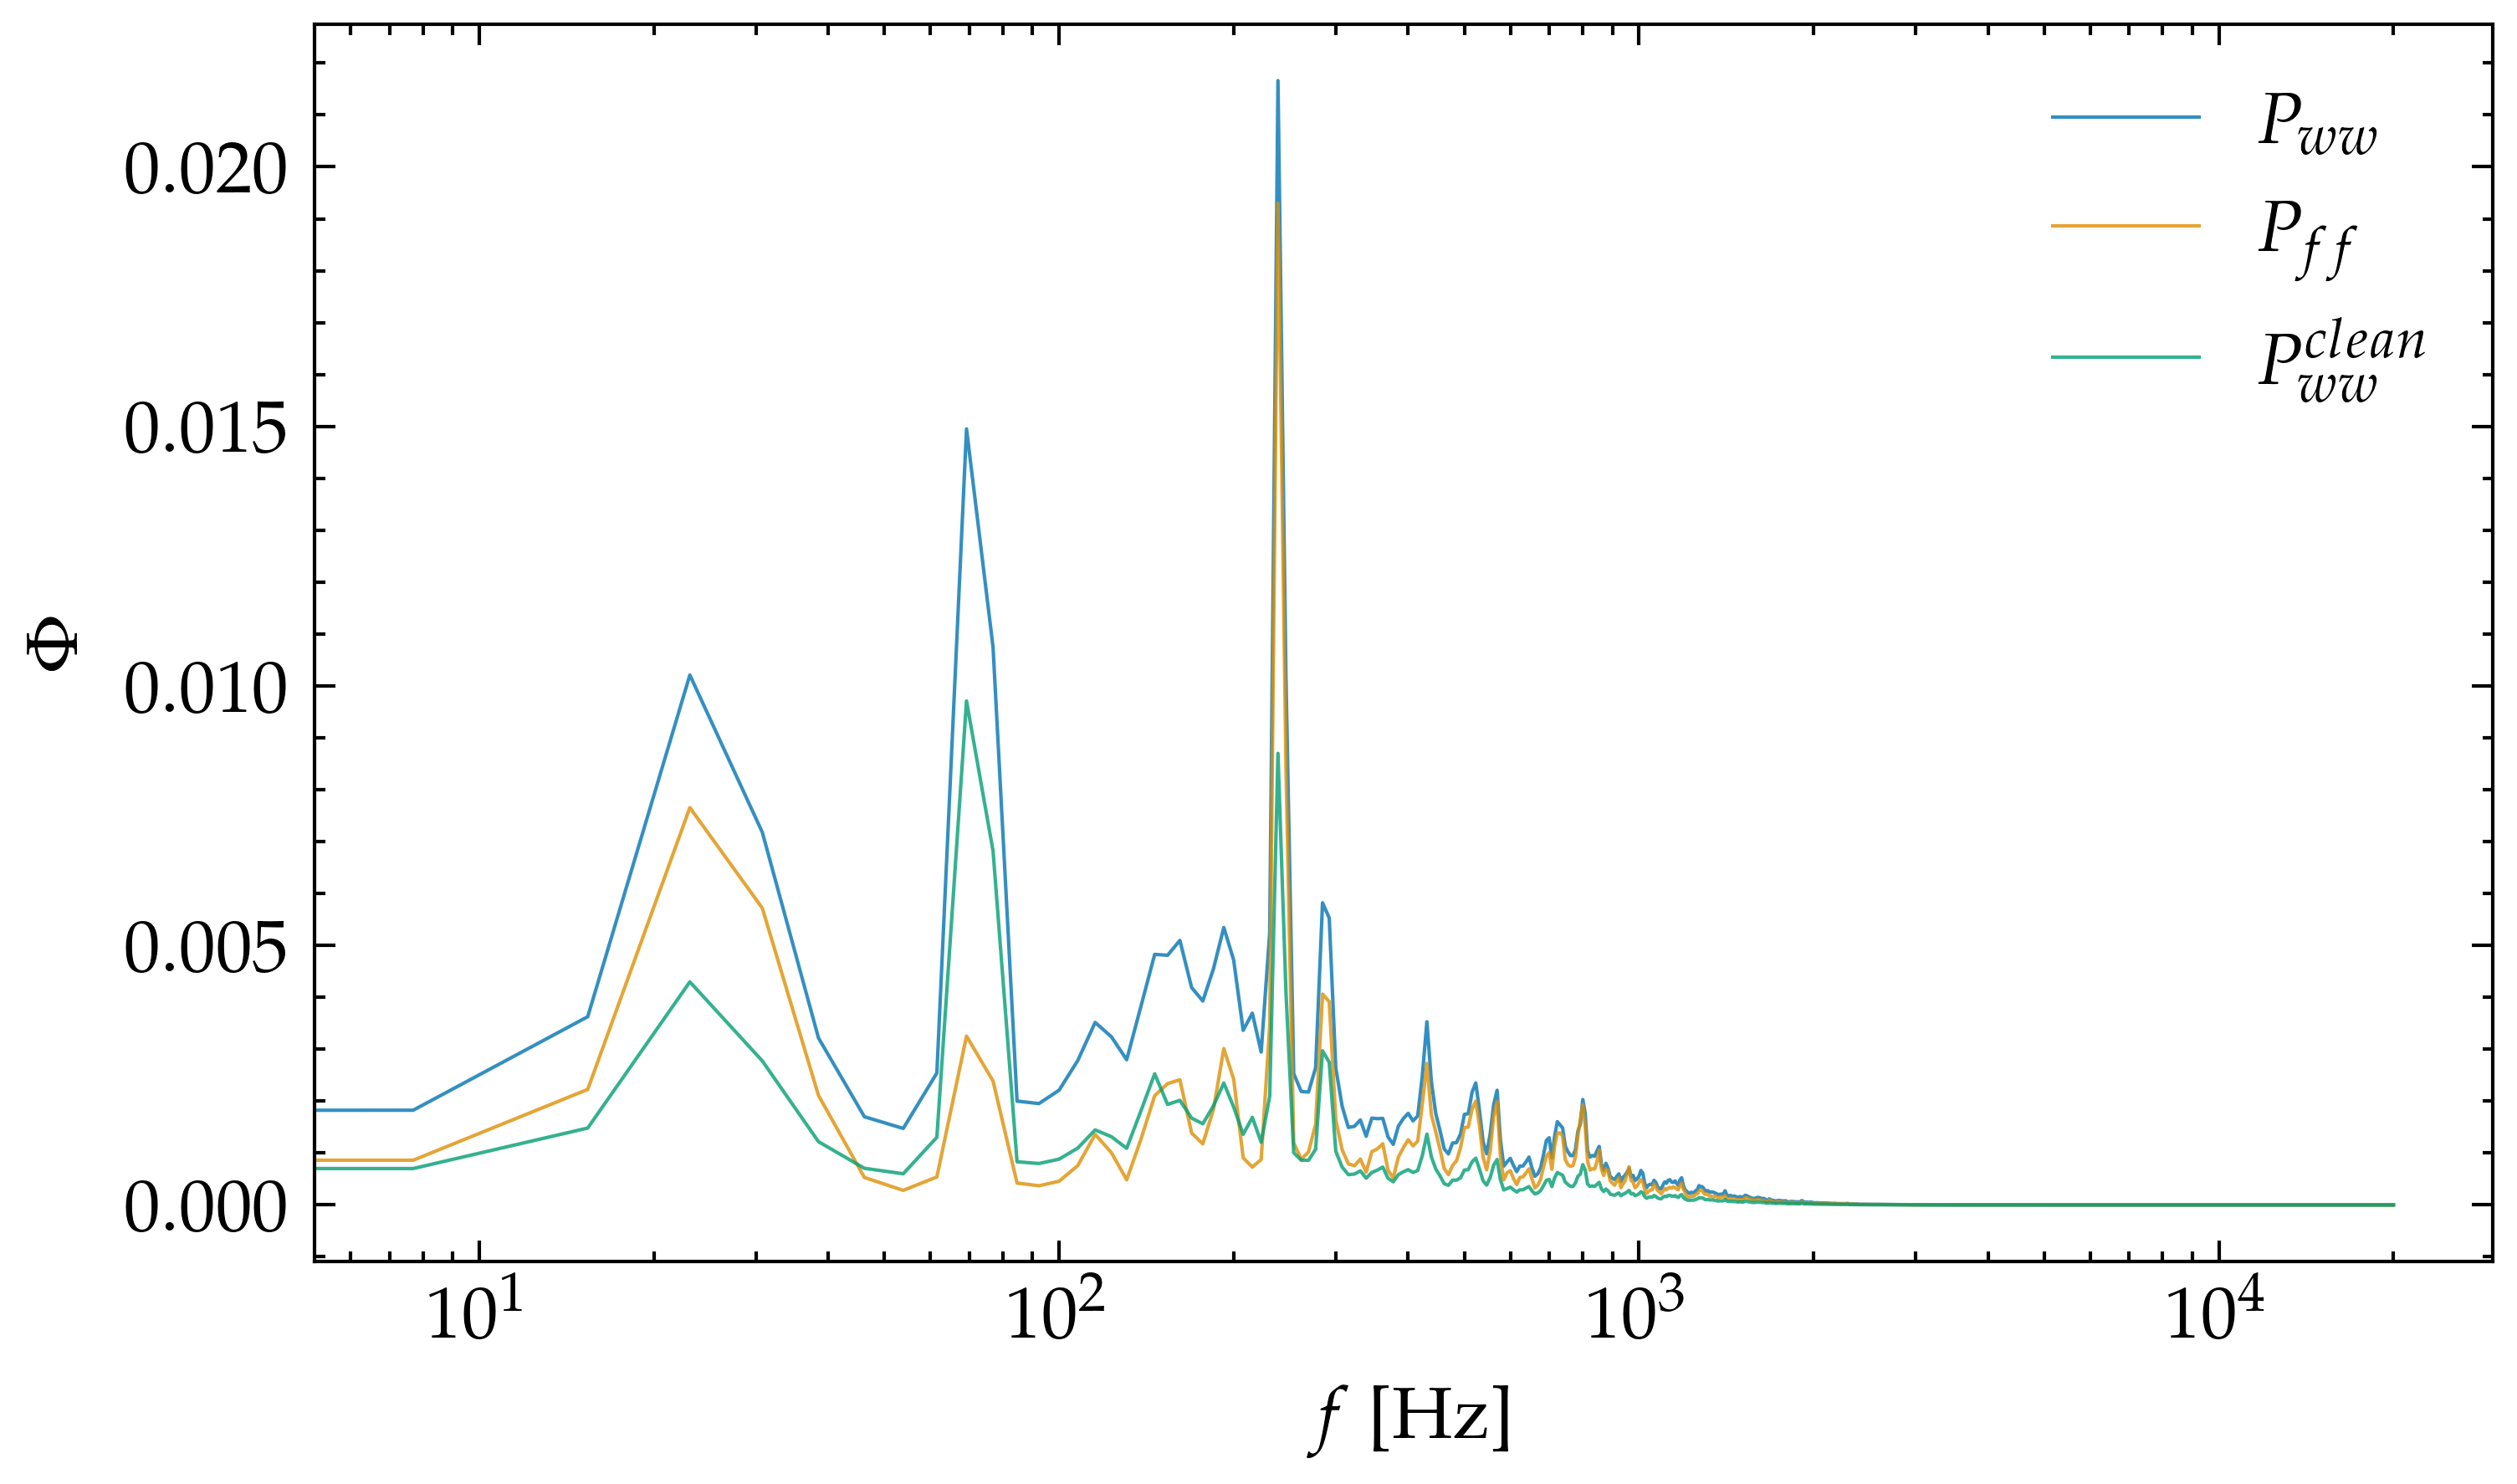
\includegraphics[width=\linewidth]{figures/wiener_filtered_spectrum.png}
    \end{minipage}
    \begin{minipage}{0.35\textwidth}
        \centering
        \begin{itemize}
            \item Duct modes \emph{should} be removed by the Wiener filter
            \item Need $|H_{wf}(f)|$ for this
        \end{itemize}
    \end{minipage}
\end{frame}


\begin{frame}{Transfer function between reference spectra and measurements}
    \centering
    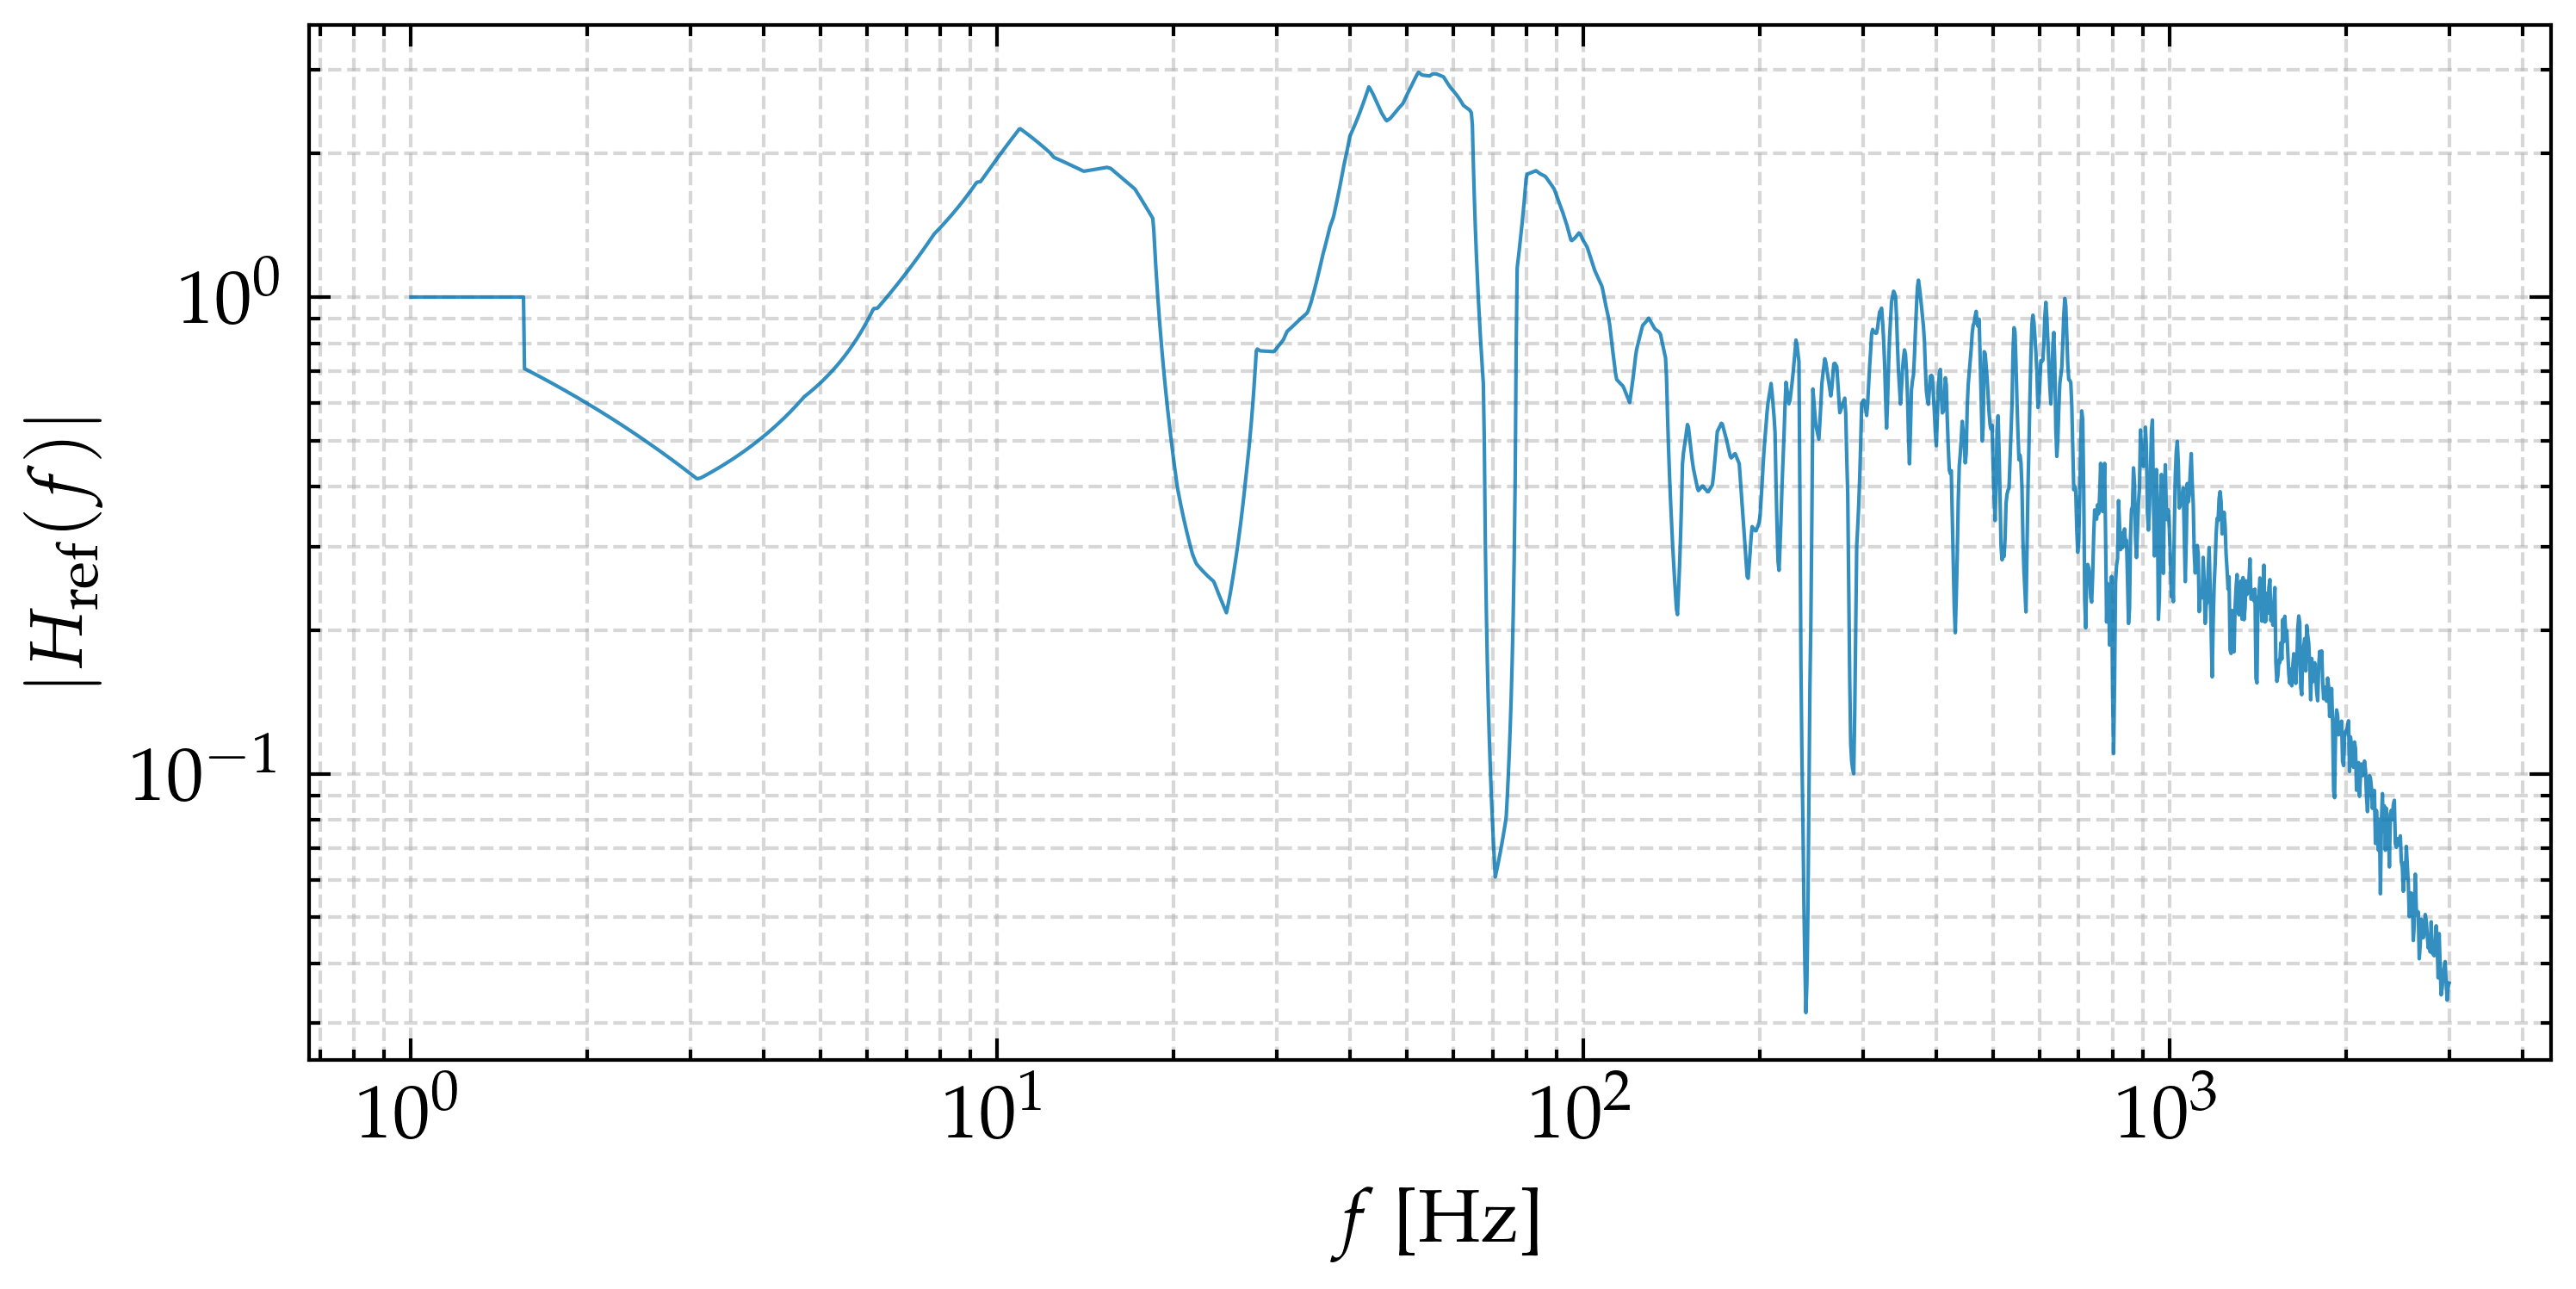
\includegraphics[width=0.7\linewidth]{figures/reference_transfer_function.png}
    \begin{itemize}
        \centering
        \item Transfer function between reference spectrum \citep{deshpande_active_2025} and current measurements
        \item Duct modes show up through the troughs of the transfer function
    \end{itemize}
\end{frame}

\begin{frame}{Corrected signals}
    \centering
    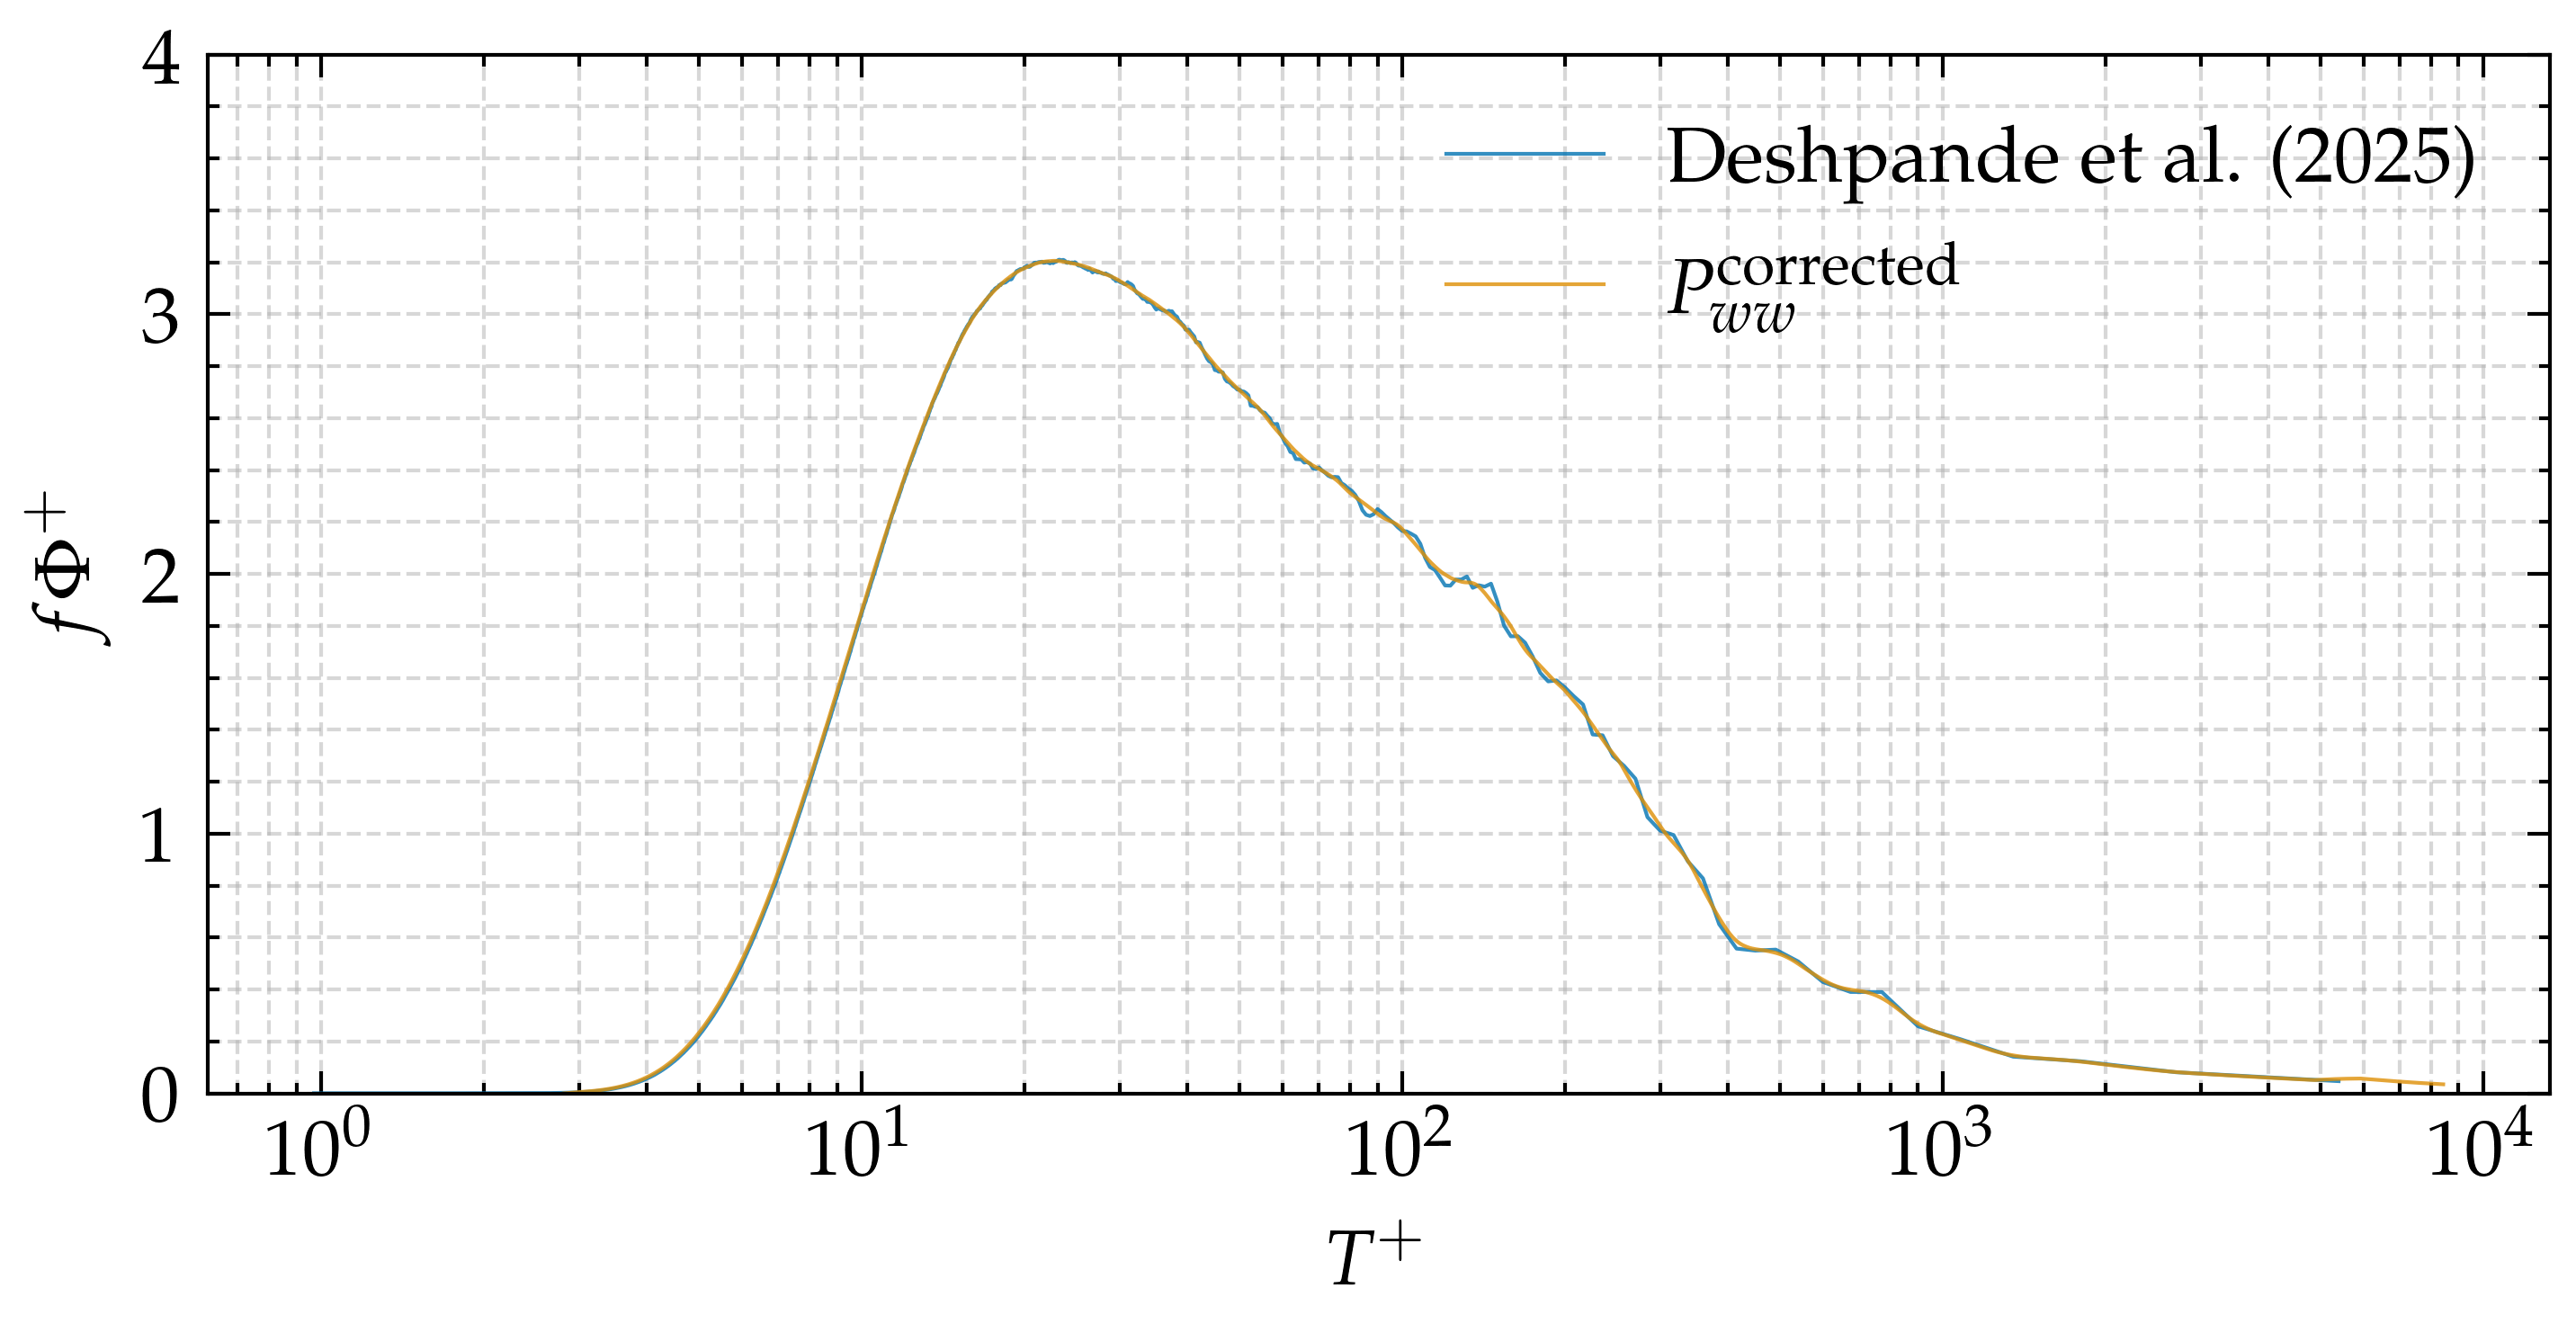
\includegraphics[width=0.7\linewidth]{figures/final_spectrum.png}
    \begin{itemize}
        \centering
        \item Corrected wall pressure signal spectrum will always match the reference spectrum
        \item We need the actual transfer function to do this
        \item Pressurising the facility will likely change the transfer function
    \end{itemize}
\end{frame}

\begin{frame}[noframenumbering,allowframebreaks]
    \frametitle{References}
    \bibliographystyle{jfm}
    \bibliography{refs}
\end{frame}

\end{document}
